
\documentclass{article}
\usepackage[utf8]{inputenc}
\usepackage{geometry}
% \geometry{a4paper,top=3cm,bottom=3cm,left=3.5cm,right=3.5cm}% heightrounded,bindingoffset=5mm}
\usepackage{array}
\usepackage{booktabs}
\usepackage{graphicx}
\usepackage{amsmath}
\usepackage{mathtools}
\usepackage{mathrsfs}
\usepackage{longtable}
\usepackage{textcomp}


\begin{document}

    Guidolin Giacomo - IN0501058 \\


    \textbf{BASI DI DATI - Registro per studiare uno strumento}\\

    \section{PROGETTAZIONE CONCETTUALE }

    \subsection{Analisi dei requisiti}

    Si vuole creare una base di dati per aiutare dei musicisti nel loro percorso di studio di un brano.\\
    I vari brani che verrano inseriti nel database possederanno un nome, un autore e avranno la possibilità di essere associati ad informazioni quali l'editore specifico dello spartito,
    l'anno di publicazione e un link per trovarne la copia online. Presenteranno anche, se possibile, dei commenti per facilitarne l'approccio stilistico al momento dello studio e una serie
    di link che rimandino a dei video su youtube per poter ascoltare altri interpreti del brano.\\
    Gli utenti della base di dati potranno, una volta cominciato lo studio, segnarsi, sulle battute che stanno approcciando, la velocità di esecuzione e eventuali commenti sulla sezione.\\
    L'utente dovrà essere in grado, se desidera di ricavare informazioni sull'autore per poter al meglio interpretare il brano.\\
    Il compositore del pezzo infatti, oltre al nome, potrà avere informazioni quali la data di nascita, la eventuale data di morte e la corrente artistica cui fa parte. Se necessario sarà anche
    possibile avere una sezione commenti per poter anche qui descrivere informazioni stilistiche tipiche del dato autore.\\
    Anche il movimento artistico, cui fa parte l'autore, presenterà alcune info quali il nome, le caratteristiche tecniche-stilistiche che la rendono una corrente a se stante,
    e se necessario il range di anni su cui si sviluppò  maggiormente.
    \\Al movimento aggiungiamo anche notizie storiche, sotto forma di eventi decisivi per lo sviluppo della corrente, che potranno essere registrati tramite nome e anno di appartenenza.
    \\In ultimo richiediamo di aggiungere una lista di strumenti musicali che saranno di tipi diversi e di case produttrici differenti dei quali l'utente ne possederà almeno uno. Questo, al
    momento dell'iscrizione, dovrà fornire dati utili quali il nome, la data di nascita e l'anno di inizio del suo percorso musicale.\\

    \subsection{Glossario dei termini}


    \begin{tabular}{l p{5cm} l p{2cm} l l}
        \toprule
        \textbf{\textit{Termine}} & \textbf{\textit{Descrizione}} & \textbf{\textit{Sinonimi}} & \textbf{\textit{Collegamenti}} \\
        \midrule
        Autore & Colui che ha prodotto un opera artistica. & Compositore & Brano, \newline Movimento \\
        \midrule
        Brano & Parte più o meno estesa di una composizione musicale. & Spartito, \newline  Pezzo  & Autore, \newline Utente, \newline Url, \newline Battuta \\
        \midrule
        Battuta & Unità di tempo rappresentata sulla partitura tramite uno spazio compreso tra due stanghette. & Sezione & Utente, \newline Brano \\
        \midrule
        Movimento & Insieme di regole stilistiche e tecniche che riguardano un periodo artistico & Corrente & Autore, \newline Eventi \\
        \bottomrule
    \end{tabular}

    \subsection{Suddivisione del testo in frasi omogenee}

    \subsubsection{Frasi di carattere generale}

    Si vuole creare una base di dati per aiutare dei musicisti nel loro percorso di studio di un brano.\\

    \subsubsection{Frasi relative al brano}

    I vari brani che verrano inseriti nel database possederanno un nome, un autore e avranno la possibilità di essere associati ad informazioni quali l'editore specifico dello spartito,
    l'anno di publicazione e un link per trovarne la copia online. Presenteranno anche, se possibile, dei commenti per facilitarne l'approccio stilistico al momento dello studio e una serie
    di link che rimandino a dei video su youtube per poter ascoltare altri interpreti del brano.\\ \\
    L'utente dovrà essere in grado, se desidera di ricavare informazioni sull'autore per poter al meglio interpretare il brano.\\


    \subsubsection{Frasi relative alle battute}

    Gli utenti della base di dati potranno, una volta cominciato lo studio, segnarsi, sulle battute che stanno approcciando, la velocità di esecuzione e eventuali commenti sulla sezione.\\

    \subsubsection{Frasi relative all'autore}

    L'utente dovrà essere in grado, se desidera di ricavare informazioni sull'autore per poter al meglio interpretare il brano.\\
    Il compositore del pezzo infatti, oltre al nome, potrà avere informazioni quali la data di nascita, la eventuale data di morte e la corrente artistica cui fa parte. Se necessario sarà anche
    possibile avere una sezione commenti per poter anche qui descrivere informazioni stilistiche tipiche del dato autore.\\ \\
    Anche il il movimento artistico, cui fa parte l'autore [\dots]\\

    \subsubsection{Frasi relative al movimento}

    Anche il il movimento artistico, cui fa parte l'autore, presenterà alcune info quali il nome, le caratteristiche tecniche-stilistiche che la rendono una corrente a se stante,
    e se necessario il range di anni su cui si sviluppò  maggiormente.\\ \\
    Al movimento aggiungiamo anche notizie storiche[\dots]\\

    \subsubsection{Frasi relative agli eventi}

    Al movimento aggiungiamo anche notizie storiche, sotto forma di eventi decisivi per lo sviluppo della corrente, che potranno essere registrati tramite nome e anno di appartenenza.

    \subsubsection{Frasi relative agli strumenti}

    In ultimo richiediamo di aggiungere una lista di strumenti musicali che saranno di tipi diversi e di case produttrici differenti dei quali l'utente ne possederà almeno uno.

    \subsubsection{Frasi relative all'utente}

    [\dots]dei quali l'utente ne possederà almeno uno. Questo, al
    momento dell'iscrizione, dovrà fornire dati utili quali il nome, la data di nascita e l'anno di inizio del suo percorso musicale.\\

    \subsection{Dizionario delle entità}

    \begin{tabular}{l p{5cm} p{3cm} p{2cm} l l l}
        \toprule
        \textbf{\textit{Entità}} & \textbf{\textit{Descrizione}} & \textbf{\textit{Attributi}} & \textbf{\textit{Identificatore}} \\
        \midrule
        Strumento & Oggetto in grado di emettere suoni. Viene utilizzato per fare musica. & Produttore, \newline Tipo, \newline ID & ID \\
        \midrule
        Utente & Il musicista che usufruisce della base di dati. & ID, \newline Nome, \newline Nascita, \newline Inizio & ID \\
        \midrule
        Brano & Parte più o meno estesa di una composizione musicale. & Nome, \newline Editore, \newline Anno, \newline Copia, \newline Commento, \newline ID, \newline URL & ID \\
        \midrule
        Battuta & Unità di tempo rappresentata sulla partitura tramite uno spazio compreso tra due stanghette & Numero, \newline Btm, \newline Commento & Numero, \newline Appartenenza \\
        \midrule
        Autore & Colui che ha prodotto un opera artistica & Nascita, \newline Morte, \newline Commento,  \newline Nome, \newline ID & ID \\
        \midrule
        Movimento & Corrente artistica & Range, \newline Caratteristiche, \newline Nome & Nome \\
        \midrule
        Evento & Evento che merita di essere tramandato per la sua importanza & Anno, \newline Nome & Nome \\
        \bottomrule
    \end{tabular}

    \subsection{Dizionario delle relazioni}

    \begin{tabular}{l p{5cm} p{3cm} p{2cm} l l l}
        \toprule
        \textbf{\textit{Relazioni}} & \textbf{\textit{Descrizione}} & \textbf{\textit{Componenti}} & \textbf{\textit{Attributi}} \\
        \midrule
        Possesso & Lo strumento è proprietà di un utente & Strumento, \newline Utente & \\
        \midrule
        Raccoglitore & Insieme di brani che un utente può o ha già studiato & Utente, \newline Brano & \\
        \midrule
        Studio & L'utente elebora in modo dettagliato e personale un brano al fine di riuscire a suonarlo & Battuta, \newline Utente & \\
        \midrule
        Appartenenza & Una battuta fa parte di un insieme di battute, il cosidetto brano & Brano, \newline Battuta & \\
        \midrule
        Compositore & Artista che produce un opera musicale & Brano, \newline Autore & \\
        \midrule
        Stile & Caratteristiche tecnico artistche riguradanti l'interpretazione storicamente accurata & Autore, \newline Movimento \\
        \midrule
        Influenza & Un movimento artistico viene definito dagli eventi storici accaduti durante il suo tempo & Movimento, \newline Evento & \\
        \bottomrule
    \end{tabular}

    \newpage

    \subsection{Modello ER}

    Coerentemente con quanto appena detto, si giunge alla formulazione del seguente modello entità-relazione:

    \begin{center}
        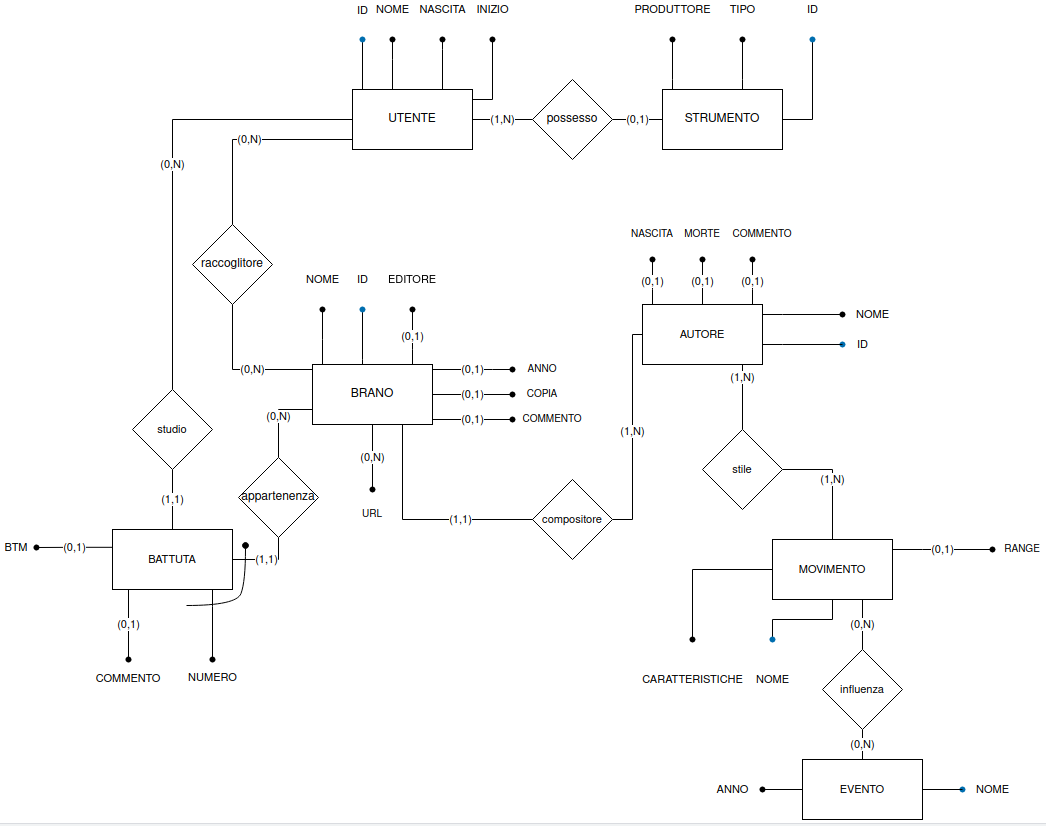
\includegraphics[width=\linewidth]{immagini/01_diagrammaER.png}   % [width=0.8\linewidth, height=0.4\textheight]{immagini/01_diagrammaER.jpg}
    \end{center}

    \subsection{Vincoli non esprimibili}

    \begin{itemize}
        \item L'anno di nascita dell'autore non può essere maggiore dell'anno attuale
        \item L'anno di nascita dell'utente non può essere maggiore dell'anno attuale
        \item L'utente non può avere più di 120 anni
        \item Il range del movimento non può avere un termine definito in anni futuri
        \item Gli eventi devono essersi svolti nel passato
    \end{itemize}

    \section{PROGGETTAZIONE LOGICA}

    \subsection{Tavola dei volumi}

    \begin{center}
        \begin{tabular}{lll}
            \toprule
            \textbf{\textit{Concetto}} & \textbf{\textit{Tipo}} & \textbf{\textit{Volume}}\\
            \midrule
            Strumento & Entità & 150\\
            \midrule
            Possesso & Relazione & 150\\
            \midrule
            Utente & Entità & 100\\
            \midrule
            Raccoglitore & Relazione & 500\\
            \midrule
            Brano &  Entità & 500\\
            \midrule
            Studio & Relazione & 250000\\
            \midrule
            Battuta &  Entità & 250000\\
            \midrule
            Compositore & Relazione & 500\\
            \midrule
            Autore &  Entità & 30\\
            \midrule
            Stile & Relazione & 30\\
            \midrule
            Movimento &  Entità & 10\\
            \midrule
            Influenza & Relazione & 200\\
            \midrule
            Evento &  Entità & 200\\
            \midrule
            Appartenenza & Relazione & 250000\\
            \bottomrule
        \end{tabular}
    \end{center}

    \subsection{Valutazione del costo}

    \begin{center}
        \begin{tabular}{ p {5cm} lll}
            \toprule
            \textbf{\textit{Operazione}} & \textbf{\textit{Tipo}} & \textbf{\textit{Frequenza}} \\
            \midrule
            Aggiunta utente & Interattiva & 10/anno \\
            \midrule
            Aggiunta brano & Interattiva & 10/mese\\
            \midrule
            Aggiunta battuta & Batch & 200/giorno\\
            \midrule
            Aggiornamento battuta & Interattiva & 800/giorno\\
            \midrule
            Prelevare informazioni tecnico-stilistiche sul brano & Interattiva & 50/mese\\
            \midrule
            Prelevare informazioni sul brano e sull'autore & Interattiva & 10/mese\\
            \midrule
            Prelevare informazioni sulle battute di un brano di un utente & Interattiva & 10/giorno\\
            \midrule
            Preleva i brani di ogni utente ordinati in base al maggior numero di battute studiate & Batch & 200/giorno\\
            \bottomrule
        \end{tabular}
    \end{center}

    \subsection{Analisi delle rindondanze}

    Si osserva che è presente una rindondanza dovuta ad un ciclo che coinvolge le entità Utente, Brano, Battuta e le relazioni Studio, Appartenenza, Raccoglitore.\\
    Si decide di andare a vedere se eliminare la relazione Raccoglitore possa influire in maniera positiva sul numero di accessi. Si vanno quindi a studiare le operazioni che coinvolgono tale relazione.\\

    \subsubsection{Prelevare informazioni sulle battute di un brano di un utente}

    \begin{center}
        \begin{tabular}{ p {5cm} llll}
            \toprule
            \multicolumn{4}{l}{\textbf{Presenza di rindondanza}}\\
            \midrule
            \midrule
            \textbf{\textit{Concetto}} & \textbf{\textit{Costrutto}} & \textbf{\textit{Accessi}} & \textbf{\textit{Tipo}}\\
            \midrule
            Battuta & E & 500 & L\\
            \midrule
            Brano & E & 1 & L\\
            \midrule
            Utente & E & 1 & L\\
            \midrule
            Studio & R & 500 & L\\
            \midrule
            Appartenenza & R & 500 & L\\
            \midrule
            Raccoglitore & R & 1 & L\\
            \midrule
            \midrule
            \textit{Accessi totali:} & & & 1503\\
            \bottomrule
        \end{tabular}
    \end{center}

    \begin{center}
        \begin{tabular}{ p {5cm} llll}
            \toprule
            \multicolumn{4}{l}{\textbf{Assenza di rindondanza}}\\
            \midrule
            \midrule
            \textbf{\textit{Concetto}} & \textbf{\textit{Costrutto}} & \textbf{\textit{Accessi}} & \textbf{\textit{Tipo}}\\
            \midrule
            Battuta & E & 500 & L\\
            \midrule
            Brano & E & 1 & L\\
            \midrule
            Utente & E & 1 & L\\
            \midrule
            Studio & R & 500 & L\\
            \midrule
            Appartenenza & R & 500 & L\\
            \midrule
            \midrule
            \textit{Accessi totali:} & & & 1502\\
            \bottomrule
        \end{tabular}
    \end{center}

    \subsubsection{Preleva i brani di ogni utente ordinati in base al maggior numero di battute studiate}

    \begin{center}
        \begin{tabular}{ p {5cm} llll}
            \toprule
            \multicolumn{4}{l}{\textbf{Presenza di rindondanza}}\\
            \midrule
            \midrule
            \textbf{\textit{Concetto}} & \textbf{\textit{Costrutto}} & \textbf{\textit{Accessi}} & \textbf{\textit{Tipo}}\\
            \midrule
            Battuta & E & 2500 & L\\
            \midrule
            Brano & E & 5 & L\\
            \midrule
            Utente & E & 1 & L\\
            \midrule
            Studio & R & 2500 & L\\
            \midrule
            Appartenenza & R & 2500 & L\\
            \midrule
            Raccoglitore & R & 5 & L\\
            \midrule
            \midrule
            \textit{Accessi totali:} & & & 7511\\
            \bottomrule
        \end{tabular}
    \end{center}

    \begin{center}
        \begin{tabular}{ p {5cm} llll}
            \toprule
            \multicolumn{4}{l}{\textbf{Assenza di rindondanza}}\\
            \midrule
            \midrule
            \textbf{\textit{Concetto}} & \textbf{\textit{Costrutto}} & \textbf{\textit{Accessi}} & \textbf{\textit{Tipo}}\\
            \midrule
            Battuta & E & 2500 & L\\
            \midrule
            Brano & E & 5 & L\\
            \midrule
            Utente & E & 1 & L\\
            \midrule
            Studio & R & 2500 & L\\
            \midrule
            Appartenenza & R & 2500 & L\\
            \midrule
            \midrule
            \textit{Accessi totali:} & & & 7506\\
            \bottomrule
        \end{tabular}
    \end{center}

    \subsubsection{Aggiunta battuta}

    \begin{center}
        \begin{tabular}{ p {5cm} llll}
            \toprule
            \multicolumn{4}{l}{\textbf{Presenza di rindondanza}}\\
            \midrule
            \midrule
            \textbf{\textit{Concetto}} & \textbf{\textit{Costrutto}} & \textbf{\textit{Accessi}} & \textbf{\textit{Tipo}}\\
            \midrule
            Battuta & E & 1 & S\\
            \midrule
            Brano & E & 1 & L\\
            \midrule
            Utente & E & 1 & L\\
            \midrule
            Studio & R & 1 & S\\
            \midrule
            Appartenenza & R & 1 & S\\
            \midrule
            Raccoglitore & R & 1 & L\\
            \midrule
            \midrule
            \textit{Accessi totali:} & & & 9\\
            \bottomrule
        \end{tabular}
    \end{center}

    \begin{center}
        \begin{tabular}{ p {5cm} llll}
            \toprule
            \multicolumn{4}{l}{\textbf{Assenza di rindondanza}}\\
            \midrule
            \midrule
            \textbf{\textit{Concetto}} & \textbf{\textit{Costrutto}} & \textbf{\textit{Accessi}} & \textbf{\textit{Tipo}}\\
            \midrule
            Battuta & E & 1 & S\\
            \midrule
            Brano & E & 1 & L\\
            \midrule
            Utente & E & 1 & L\\
            \midrule
            Studio & R & 1 & S\\
            \midrule
            Appartenenza & R & 1 & S\\
            \midrule
            \midrule
            \textit{Accessi totali:} & & & 8\\
            \bottomrule
        \end{tabular}
    \end{center}

    \subsubsection{Analisi convenienza}

    Tenendo conto del numero di accessi al giorno si ottiene un miglioramento di 1210 accessi totali. Anche se non risulta essere una differenza elevata si decide di eliminare la rindondanza, ipotizzando un futuro accrescimento del database che
    aumenterebbe la dimensione del sopracitato miglioramento.\\

    \subsection{Eliminazione delle generalizzazioni}

    Non sono presenti generalizzazioni da poter eliminare.\\

    \subsection{Analisi degli attributi multivalore}

    Si può notare la presenza di un attributo multivalore nell'entità Brano, andiamo quindi a eliminarlo aggiungendo l'entità URL.

    \subsection{Presentazione modello E-R ristrutturato}

    A seguito delle considerazioni sopra elencate, si è rielaborato un nuovo modello entità-relazioni di seguito mostrato:

    \begin{center}
        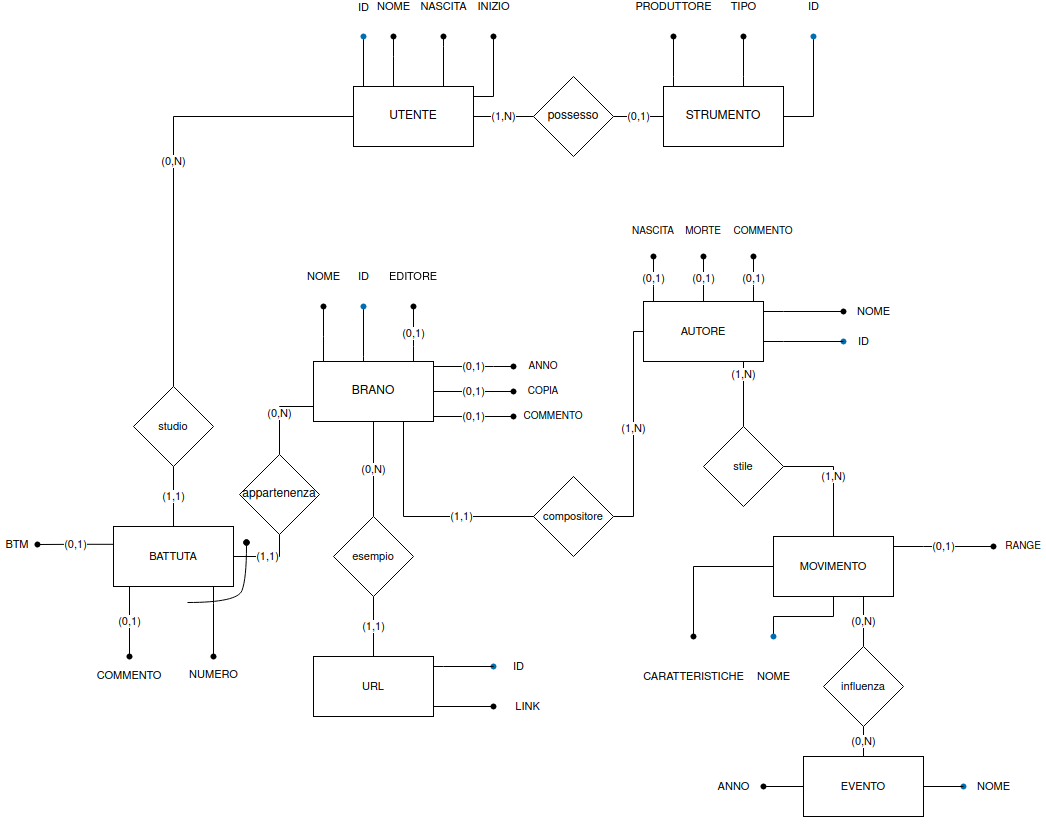
\includegraphics[width=\linewidth]{immagini/02_diagrammaER.png}
    \end{center}

    \subsection{Scelta degli identificatori primari}

    Come identificatori primari sono stati scelti:
    \begin{center}
        \begin{tabular}{ p {5cm} ll}
            \toprule
            \textbf{\textit{Chiave primaria}} & \textbf{\textit{Attributo}}\\
            \midrule
            Strumento & ID\\
            \midrule
            Utente & ID\\
            \midrule
            Battuta & Numero e Brano (identificatore esterno)\\
            \midrule
            Brano & ID\\
            \midrule
            URL & ID\\
            \midrule
            Autore & ID\\
            \midrule
            Movimento & Nome\\
            \midrule
            Evento & Nome\\
            \bottomrule
        \end{tabular}
    \end{center}

    \subsection{Passaggio al modello relazionale}

    Si individuano le seguenti relazioni, identificatori e attributi per lo schema logico con il
    modello relazionale:

    \begin{itemize}
        \item Strumento(\underline{ID}, Produttore, Tipo, Utente);
        \item Utente(\underline{ID}, Nome, Nascita, Inizio);
        \item Battuta(\underline{Numero}, \underline{Brano}, BTM, Commento, Utente);
        \item Brano(\underline{ID}, Nome, Editore, Anno, Copia, Commento, Autore);
        \item URL(\underline{ID}, Link, Brano);
        \item Autore(\underline{ID}, Nascita, Morte, Commento, Nome);
        \item Stile(\underline{Autore}, \underline{Movimento});
        \item Movimento(\underline{Nome}, Caratteristiche, Range);
        \item Influenza(\underline{Movimento}, \underline{Evento});
        \item Evento(\underline{Nome}, Anno).
    \end{itemize}

    \subsection{Modello logico}

    In accordo con tutte le considerazioni espresse, il modello logico formulato è il seguente:

    \begin{center}
        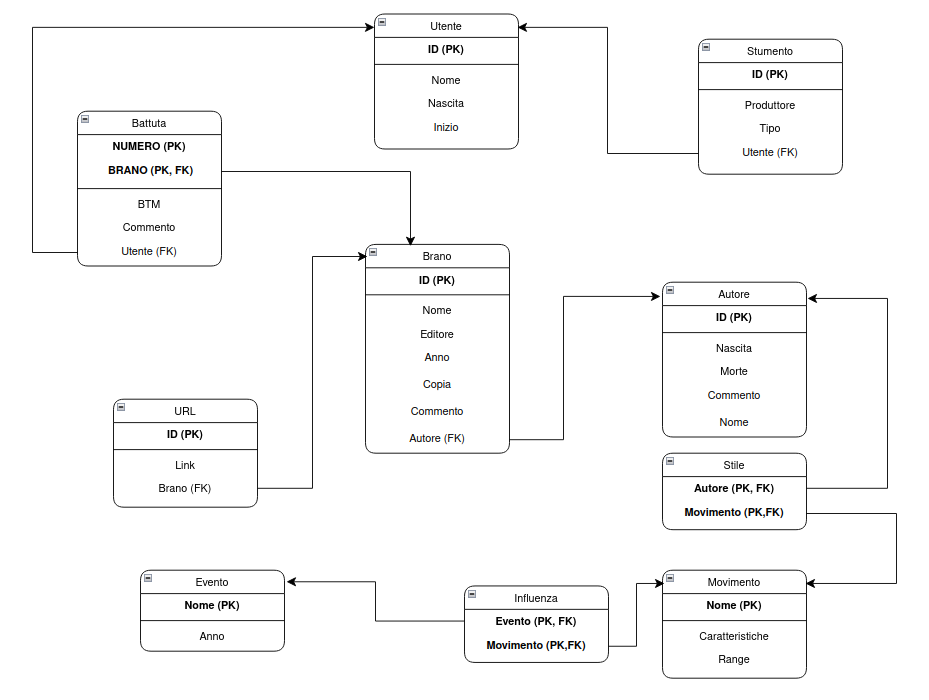
\includegraphics[width=\linewidth]{immagini/logico.png}
    \end{center}

    \subsection{Normalizzazione}

    Il database proposto:
    \begin{itemize}
        \item \'E in prima forma normale: tutte le colonne sono atomiche, non sono presenti unità ripetitive
        \item \'E in seconda forma normale: ogni tabella memorizza solamente dati relativi alla entità descritta dalla primary key. Non occorre attuare un procedimento di decomposizione.
        \item \textbf{Non è in terza forma normale}: Si può discutere sulla dipendenza della colonna Copia dalle colonne Nome, Editore e Anno.
    \end{itemize}

    Si sceglie di non completare la normalizzazione e di lasciare stare la terza forma normale. Tentare di eliminare la denormalizzazione risulterebbe un lavoro inultile, perchè per definizione
    del database non risulterà mai necessario modificare le colonne Nome, Editore e Anno, poichè lo studio di un brano risulterà collegato strettamente all'edizione utilizzata.

    \section{Realizzazione ottimizzazioni}

    \subsection{Create da eliminare}

    \begin{verbatim}
        CREATE DATABASE musica;

        USE musica;

        CREATE TABLE Utente (
                                ID INT AUTO_INCREMENT PRIMARY KEY,
                                Nome VARCHAR(50) NOT NULL,
                                Nascita DATE NOT NULL ,
                                Inizio DATE NOT NULL
        );

        CREATE TABLE Autore (
                                ID INT AUTO_INCREMENT PRIMARY KEY,
                                Nome VARCHAR(50) NOT NULL,
                                Nascita DATE,
                                Morte DATE,
                                Commento TEXT
        );

        CREATE TABLE Brano (
                               ID INT AUTO_INCREMENT PRIMARY KEY,
                               Nome VARCHAR(100) NOT NULL,
                               Editore VARCHAR(100),
                               Anno INT,
                               Copia INT,
                               Commento TEXT,
                               Autore INT,
                               FOREIGN KEY (Autore) REFERENCES Autore(ID)
        );

        CREATE TABLE Strumento (
                           ID INT AUTO_INCREMENT PRIMARY KEY,
                           Produttore VARCHAR(50) NOT NULL ,
                           Tipo VARCHAR(50) NOT NULL ,
                           Utente INT,
                           FOREIGN KEY (Utente) REFERENCES Utente(ID)
        );


        CREATE TABLE Battuta (
                                 Numero INT,
                                 Brano INT,
                                 BTM INT,
                                 Commento TEXT,
                                 Utente INT,
                                 PRIMARY KEY (Numero, Brano),
                                 FOREIGN KEY (Brano) REFERENCES Brano(ID),
                                 FOREIGN KEY (Utente) REFERENCES Utente(ID)
        );

        CREATE TABLE URL (
                             ID INT AUTO_INCREMENT PRIMARY KEY,
                             Link TEXT NOT NULL ,
                             Brano INT,
                             FOREIGN KEY (Brano) REFERENCES Brano(ID)
        );

        CREATE TABLE Movimento (
                                   Nome VARCHAR(50) PRIMARY KEY,
                                   Caratteristiche TEXT NOT NULL,
                                   'Range' VARCHAR(50)
        );

        CREATE TABLE Stile (
                               Autore INT,
                               Movimento VARCHAR(50),
                               PRIMARY KEY (Autore, Movimento),
                               FOREIGN KEY (Autore) REFERENCES Autore(ID),
                               FOREIGN KEY (Movimento) REFERENCES Movimento(Nome)
        );

        CREATE TABLE Evento (
                                Nome VARCHAR(100) PRIMARY KEY,
                                Anno INT NOT NULL
        );

        CREATE TABLE Influenza (
                           Movimento VARCHAR(50),
                           Evento VARCHAR(100),
                           PRIMARY KEY (Movimento, Evento),
                           FOREIGN KEY (Movimento) REFERENCES Movimento(Nome),
                           FOREIGN KEY (Evento) REFERENCES Evento(Nome)
        );



    \end{verbatim}
    
    \subsection{Aggiunta utente}
    
    \begin{verbatim}
        DELIMITER $$

        CREATE PROCEDURE addUtente(
            IN newNome VARCHAR(50),
            IN newNascita DATE,
            IN newInizio DATE,
            IN StrumentoID INT
        )
        BEGIN
            -- Variabile per memorizzare l'ID del nuovo utente
            DECLARE UtenteID INT;

            -- Inserisce il nuovo utente nella tabella Utente
            INSERT INTO Utente (Nome, Nascita, Inizio)
            VALUES (newNome, newNascita, newInizio);

            -- Ottiene l'ID dell'utente appena inserito
            SET UtenteID = LAST_INSERT_ID();

            -- Aggiorna la tabella Strumento per associare lo strumento all'utente
            UPDATE Strumento
            SET Utente = UtenteID
            WHERE ID = StrumentoID;

        END $$

        DELIMITER ;

    \end{verbatim}
    
    \subsection{Aggiunta brano}
    
    \begin{verbatim}
        DELIMITER $$

        CREATE PROCEDURE addBrano(
            IN newNome VARCHAR(100),
            IN newEditore VARCHAR(100),
            IN newAnno INT,
            IN newCopia INT,
            IN newCommento TEXT,
            IN AutoreID INT
        )
        BEGIN
            -- Inserisce il nuovo brano nella tabella Brano
            INSERT INTO Brano (Nome, Editore, Anno, Copia, Commento, Autore)
            VALUES (newNome, newEditore, newAnno, newCopia, newCommento, AutoreID);
        END $$

        DELIMITER ;
    \end{verbatim}
    
    \subsection{Aggiornamento battuta}

\end{document}
